\chapter{Overview}

Sadulli is a tightly integrated unit that contains an electric motor with a sensorless electronic speed controller
in a single monolithic package. Sadulli supply package includes an integrated drive and a propeller.
Sadulli comes pre-tuned for its particular motor and propeller,
which ensures high-efficiency operation and excellent dynamic response.
Compact and tightly integrated design minimizes motor wiring and hence internal resistance, which, in turn,
means fewer power losses and EMI.
The controller provides up to 500 W of continuous power output and supports a wide range of operating voltages
12-33.6 V (4–8S $\text{LiCoO}_\text{2}$ battery).

Although the device comes completely pre-tuned comprehensive fine-tuning is still available to the end-user.
Zubax Sadulli is fully UAVCAN compatible and enables easy integration into the end system by
using a full set of standard UAVCAN Micro connectors
\footnote{For more details refer to \url{https://uavcan.org/Specification/8._Hardware_design_recommendations/}}.

Zubax Sadulli constantly measures and reports all the crucial variables during operation
(like the controller’s temperature, motor temperature, current consumption, battery voltage, etc.)
improving system reliability.

Zubax Sadulli is an open hardware reference design for Mitochondrik.
Mitochondrik is an integrated module (like an integrated circuit) that enables third-party hardware engineers
to design sophisticated custom motor controllers using motor control technology – T\'elega,
which integrates advanced control algorithms. This datasheet is focused only on the Sadulli hardware.

\section{System integration}
Zubax Sadulli is a single supply device, which means that the device does not expose any power supply inputs
except for the high power supply. The 5 V rails of the CAN interfaces are not used by the device;
rather, the device may provide 5 V power line for UAVCAN bus from its internal DC-DC converter if needed.

\begin{figure}[h]
    \centering
    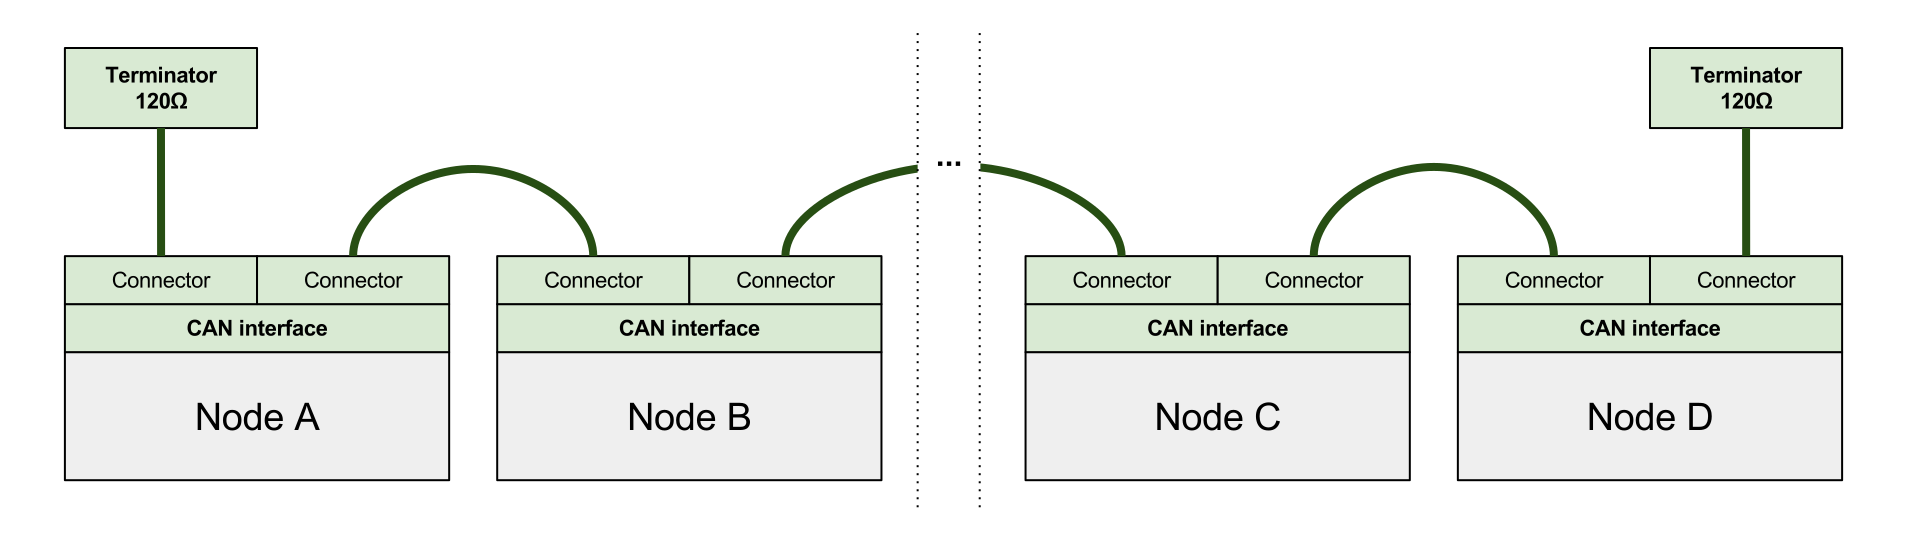
\includegraphics[width=1\textwidth]{figures/can_integration.png}
    \caption{Connection of CAN nodes}
\end{figure}

\section{Variants}

Three versions of Sadulli hardware are available:
\begin{itemize}
    \item \textbf{Sadulli Piccino} can be applied for light multirotor aircraft with takeoff mass up to 1500 g/rotor.
    \item \textbf{Sadulli Grosso} can be applied for multirotor aircraft with takeoff mass 4000 g/rotor
    \item \textbf{Sadulli Nudo} is a version of the hardware that does not include the motor and propeller
    and is supposed to be used with the vendor's motor of choice. It can also be fine-tuned for that motor if requested.
\end{itemize}

\begin{ZubaxTableWrapper}{Sadulli variants}
\begin{ZubaxWrappedTable}{| l | X | X |}
    Version     & Motor     & Propeller             \\
    Nudo        & ---       & ---                   \\
    Piccino     & V4006     & 15*55 non-foldable    \\
    Grosso      & V4014     & 17*62 foldable        \\
\end{ZubaxWrappedTable}
\end{ZubaxTableWrapper}

Both Sadulli Piccino and Grosso propellers are made out of carbon fiber filled nylon PA66.